\documentclass[12pt,letterpaper]{report}
\usepackage[utf8]{inputenc}
\usepackage{geometry}
\geometry{letterpaper, margin=1in}
\usepackage{hyperref}
\usepackage{titlesec}
\usepackage{setspace}
\usepackage{graphicx}
\usepackage{float}
\usepackage{booktabs}
\usepackage{amsmath}
\usepackage{amssymb}
\usepackage{tikz}
\usetikzlibrary{shapes.geometric, arrows.meta, positioning, fit, calc, decorations.pathreplacing}
\onehalfspacing

\begin{document}

% --- Front Matter ---
\pagenumbering{roman}

% 1. Title Page (Page i, number omitted)
\begin{titlepage}
    \centering
    \vspace*{1in}
    {\Large \bfseries NeuralFace: Generative Models for \\ Real-Time Face-to-Face Interaction \par}
    \vspace{1.5in}
    by\par
    \vspace{0.5in}
    Henry Heng Yi Lin\par
    \vspace{1.5in}
    A thesis\\
    presented to the University of Waterloo\\
    in fulfillment of the\\
    thesis requirement for the degree of\\
    Master of Mathematics\\
    in\\
    Computer Science\par
    \vspace{1in}
    Waterloo, Ontario, Canada, 2026\par
    \vspace{0.5in}
    \copyright\ Henry Heng Yi Lin 2026
\end{titlepage}

\setcounter{page}{2}

% 2. Author's Declaration
\chapter*{Author's Declaration}
\addcontentsline{toc}{chapter}{Author's Declaration}
This thesis consists of material all of which I authored or co-authored: see Statement of Contributions included in the thesis. This is a true copy of the thesis, including any required final revisions, as accepted by my examiners. 

I understand that my thesis may be made electronically available to the public.

% 3. Statement of Contributions
\chapter*{Statement of Contributions}
\addcontentsline{toc}{chapter}{Statement of Contributions}


% 4. Abstract
\chapter*{Abstract}
\addcontentsline{toc}{chapter}{Abstract}
Digital avatars could enable more expressive virtual communication, personalized AI assistants, and new forms of telepresence. However, most existing avatar-generation systems focus on producing short video clips. A digital avatar that participates in an ongoing interaction must instead generate video continuously while preserving its identity, responding naturally to speech and facial motion, and remaining visually coherent over long periods of time.

This thesis studies continuous digital avatar generation. Given a target identity and a live driving stream, the system aims to render an animated version of the target that follows the driver's expressions and behavior without inheriting the driver's appearance. We develop a recurrent diffusion-based architecture that maintains visual state across time, allowing the avatar to generate extended sequences without repeatedly processing its entire history.

Our experiments reveal that continuous generation introduces a fundamental identity-stability problem. In the baseline system, the avatar gradually loses the target's facial structure and converges toward the identity of the driving person, producing identity leakage in 93\% of evaluated sequences. We introduce explicit identity anchoring, feature-space projection, and knowledge transfer from a pretrained video model to better separate who the avatar is from how it moves. These methods eliminate observed identity leakage under teacher-forced evaluation, reducing it from 93\% to 0\%. However, identity drift can reappear during fully autoregressive generation as small visual errors accumulate over time. We also find that incorporating dense audio representations can disrupt the model's visual memory, highlighting an additional challenge for speech-driven avatars.

These results demonstrate progress toward digital avatars that can sustain a coherent visual presence throughout an interaction. They also identify long-term identity preservation, autoregressive stability, and audiovisual integration as key challenges for building persistent, real-time digital humans.

% 5. Acknowledgements
\chapter*{Acknowledgements}
\addcontentsline{toc}{chapter}{Acknowledgements}
First and foremost, I would like to express my deepest gratitude to my advisor, Professor Yuntian Deng, whose strategic guidance, rigorous academic standards, and continuous support have been instrumental in the realization of this research. I would also like to thank my peers and the systems administrators who maintained the H100 cluster infrastructure that made this continuous video generation research computationally possible.

% 6. Table of Contents
\tableofcontents

% 7. List of Figures
\listoffigures
\addcontentsline{toc}{chapter}{List of Figures}

\clearpage

% --- Main Body ---
\pagenumbering{arabic}

\chapter{Introduction}

Digital avatars hold the potential to revolutionize virtual communication, enabling personalized AI assistants and immersive telepresence. However, building a digital human that can participate in an ongoing, real-time interaction requires generating video continuously while preserving a coherent visual identity. The generation of highly photorealistic, temporally continuous video sequences remains one of the most formidable frontiers in deep generative modeling. While Latent Diffusion Models (LDMs) have demonstrated unprecedented success in high-fidelity text-to-image synthesis, extending these architectures to the temporal domain has historically been constrained by fundamental computational bottlenecks. The recent transition from U-Net based backbones to Diffusion Transformers (DiTs) has enabled greater architectural scalability and refined latent routing. However, standard DiTs rely on global self-attention mechanisms, which inherently suffer from a quadratic $O(L^2)$ computational complexity with respect to the sequence length $L$. For high-framerate, long-horizon video generation---such as the continuous, infinite-length synthesis of digital human avatars at 60 frames per second---this quadratic scaling renders deep autoregressive rollouts computationally intractable. 

This thesis investigates a novel structural paradigm designed to overcome these temporal constraints: the integration of a Structured State Space Duality (SSD) sequence mixer---specifically Mamba-2---within a Diffusion Transformer scaffold. By explicitly decoupling the generative diffusion optimization path from the recurrent temporal memory, this work presents a hybrid architecture capable of theoretically continuous video generation at a linear $O(L)$ computational complexity.

\section{The Promise of Linear Scaling and the Inductive Bias Problem}
In a traditional visual attention block, every patch in a generated frame must compute its affinity with every other patch in the historical context window. As the temporal horizon expands, the context window inevitably overflows available GPU memory limits. Structured State Space Models (SSMs), and Mamba-2 in particular, offer a mathematical alternative. By compressing the historical sequence into a fixed-size hidden state via a continuous-time selective scan, Mamba-2 allows the temporal context to be processed sequentially and linearly. 

While recent scaling laws highlight the theoretical expressiveness of state-space dimensions, applying SSMs to complex visual modalities introduces severe inductive biases. The foundational flaw in applying pure state-space models to visual diffusion paradigms lies in the inherent scanning mechanisms utilized to process multidimensional data. Mamba architectures are fundamentally designed for 1D causal sequence modeling. Forcing 2D spatial patches into a flattened 1D sequence severely disrupts spatial locality. When combined with the inherent stochasticity of diffusion processes, this often results in catastrophic \textit{exposure bias} during autoregressive inference. Without the ground-truth context to constantly correct the trajectory (as seen in teacher-forced training), minor out-of-distribution (OOD) errors in early layers rapidly compound into total structural collapse. Addressing this fragility in the latent visual manifold forms the primary technical contribution of this research.

\section{The Digital Avatar Problem: Bipartite Context and Attractor Overload}
The efficacy of the proposed Mamba-2 DiT hybrid is evaluated through the highly constrained task of Digital Avatar generation. This domain demands the precise orchestration of a dual-stream context window: the model must continuously synthesize the visual identity of a static \textit{Target Avatar} while dynamically applying the motion, structural pose, and expressions derived from a driving \textit{Source User}. 

This specific domain ruthlessly exposes the weaknesses of autoregressive sequence mixers. Unlike generic text-to-video generation, where the network can hallucinate novel geometries seamlessly and recover from temporal drift, digital avatar generation requires rigid temporal consistency. The network must hold a single, pristine geometric identity in its state-space memory across thousands of frames. Our preliminary investigations revealed a critical vulnerability in this setup, which we formalize as \textit{Conditioning Collapse} or \textit{Attractor Overload}. As the autoregressive rollout deepens, the model's selective scan mechanisms begin to conflate the dynamic motion latents of the driving source with the static geometric identity of the target. We document this phenomenon as a massive geometric bias where the generated avatar steadily morphs into the driving user's underlying bone structure due to an overwhelmingly dominant static latent attractor. 

\section{Core Contributions}
To realize the linear scaling benefits of the Mamba-2 sequence mixer without succumbing to manifold collapse, this thesis introduces a comprehensive architectural and mathematical methodology to heal the visual state-space. The core contributions of this work are three-fold:

\begin{itemize}
    \item \textbf{Formulation of the Mamba-2 DiT Hybrid and the ``Anchor-Last'' Paradigm:} We detail the implementation of a frozen long-context SSM mixer governed by trainable DiT-style conditioning (AdaLN + MLP). Furthermore, we establish the ``Anchor-Last'' context formulation, a novel structural arrangement that places the target avatar's identity grounding frame at the absolute end of the prefill window. By organizing the sequence precisely before the noisy diffusion target, we maximize SSM state grounding, ensuring the target identity can ``shout over'' residual noise during the continuous scan.
    
    \item \textbf{Mitigation of Source Identity Bleed via Latent Manifold Healing:} During initial empirical evaluation, our baseline architecture suffered a 93\% User Leakage rate. We successfully isolated and eradicated this geometric bias through two primary interventions:
    \begin{itemize}
        \item \textbf{Rank-1 Null-Space Projection:} By calculating the exact mean latent tensor for the primary driver across 952 context frames, we mathematically projected the Mamba-2 hidden states into the null-space of this mean vector. This effectively blinded the Mamba-2 backbone to the source user's static geometry, forcing the model to operate entirely in the subspace of pure motion.
        \item \textbf{Transformer-to-Mamba Feature Distillation (T2MD):} We introduced a layer-level feature matching objective via MSE loss, utilizing a frozen DiT Teacher to guide the Mamba-2 Student. Combined, these interventions stabilized the visual manifold. 
    \end{itemize}
    
    \item \textbf{Formalizing the Open Challenge of High-Variance Audio-Visual Integration:} While the visual pathways of the avatar model were successfully stabilized, the multimodal integration of high-bandwidth audio remains an immensely complex open problem for state-space models. Attempting to condition the avatar via a 32-codebook (24kbps) EnCodec audio stream introduced destructive high-variance embeddings that functioned as global noise. This effectively flushed the SSD's spatial memory. This thesis formally details the mathematical complexities of this failure mode, analyzing the impact of \textit{Latent Spatial Smearing} (where global cross-attention improperly distributes audio embeddings across the entire $H \times W$ feature map) and \textit{Stridal Desynchronization} (the phase shift caused by mapping 60fps linear EnCodec tokens against a 15fps visual sequence). We explicitly frame multimodal temporal alignment as the immediate next frontier for continuous SSM video generation.
\end{itemize}

\section{Thesis Structure}
The remainder of this thesis is structured as follows:
\begin{itemize}
    \item \textbf{Chapter 2 (Background \& Related Work)} provides the necessary theoretical foundation, reviewing the evolution of Latent Diffusion Models, the mechanics of Mamba-2, and contemporary literature on conditioning collapse and continuous sequence mixing.
    \item \textbf{Chapter 3 (Architectural Setup \& The Anchor-Last Paradigm)} details the core methodology behind our Mamba-2 DiT hybrid, exploring the state-space decoupling, computational scaling advantages, and the dual-stream context window logic.
    \item \textbf{Chapter 4 (Methodology and Visual Results: Healing the Manifold)} serves as the primary empirical core of the thesis. It documents the discovery of source identity bleed and details the successful mathematical implementations of Rank-1 Null-Space Projection and T2MD to achieve perfect identity retention under controlled settings.
    \item \textbf{Chapter 5 (Challenges in Audio-Visual Alignment: Future Work)} outlines our multimodal findings, thoroughly diagnosing the architectural disruptions caused by EnCodec audio streams, and proposing robust structural interventions (such as Spatial Bounding Box Masking) for future researchers.
    \item \textbf{Chapter 6 (Conclusion)} summarizes the contributions and contextualizes the future of state-space models in long-horizon multimodal computer vision.
\end{itemize}

\chapter{Background \& Related Work}

The pursuit of continuous, high-fidelity video generation exists at the intersection of several rapidly evolving paradigms in deep learning. This chapter reviews the foundational architectures that inform our Mamba-2 DiT hybrid model. We trace the evolution of Latent Diffusion Models (LDMs) into the temporal domain, analyze the computational bottlenecks of Diffusion Transformers (DiTs), and evaluate the recent rise of Structured State Space Models (SSMs). Finally, we examine contemporary literature surrounding conditioning collapse and exposure bias—the specific failure modes our methodology is designed to resolve.

\section{Autoregressive Video Generation and LDMs}
Latent Diffusion Models have fundamentally redefined the state-of-the-art in generative computer vision. By compressing high-dimensional pixel space into a lower-dimensional latent manifold via a Variational Autoencoder (VAE), LDMs can perform the iterative denoising process with significantly higher computational efficiency~\cite{rombach2022highresolution}. 

While highly successful in text-to-image synthesis, extending LDMs to continuous video generation introduces profound difficulties~\cite{blattmann2023align}. Standard autoregressive video generation relies on a sliding context window, where previously generated frames condition the synthesis of future frames. However, the stochastic nature of the diffusion process frequently causes minor out-of-distribution (OOD) artifacts in early frames. During deep autoregressive rollouts, these errors compound exponentially—a phenomenon known as \textit{exposure bias}~\cite{bengio2015scheduled}. Unlike natural language processing, where autoregressive token generation is heavily stabilized by a discrete vocabulary, visual manifolds are continuous, making them highly susceptible to structural drift over long horizons~\cite{statespacediffuser2025}. Furthermore, if the first-stage VAE encodes disparate visual identities too closely within the normalized latent space, the autoregressive sequence can easily blur the boundaries between distinct conditioning streams, precipitating severe geometric collapse.

\section{Diffusion Transformers (DiTs)}
Historically, LDMs have relied on U-Net backbones, which utilize spatial convolutions and downsampling~\cite{rombach2022highresolution}. Recent architectural shifts have demonstrated that replacing the U-Net with a Diffusion Transformer (DiT) yields far greater scalability and more expressive latent routing~\cite{peebles2023scalable}. DiTs patchify the latent representations and process them through deep stacks of multi-head self-attention (MHSA) and Adaptive Layer Normalization (AdaLN) blocks~\cite{peebles2023scalable}. Architecturally, a standard DiT block relies on AdaLN-Zero timestep conditioning, pre-norm modulation, and GELU Multi-Layer Perceptrons (MLPs) to effectively guide the generative path. 

The fatal limitation of the standard DiT for continuous video generation is its reliance on global self-attention~\cite{peebles2023scalable}. The self-attention mechanism scales quadratically—$O(L^2)$—with respect to the sequence length $L$. For digital avatar generation, which requires maintaining a dense historical context window at 60 frames per second, the sequence length rapidly balloons into the tens of thousands of tokens. This quadratic scaling renders continuous autoregressive video generation practically unfeasible on standard GPU hardware without severe spatial downsampling or temporal chunking~\cite{peebles2023scalable}. 

\section{Structured State Space Models (SSMs) and Mamba-2}
To circumvent the quadratic bottleneck of attention, researchers have revitalized recurrent sequence mixers, most notably through Structured State Space Models (SSMs)~\cite{gu2022efficiently}. The Mamba-2 architecture offers a highly optimized mathematical alternative~\cite{dao2024transformers}. By compressing historical context into a fixed-size hidden state via a continuous-time selective scan, Mamba-2 enables theoretically infinite sequence processing at a linear $O(L)$ computational complexity~\cite{dao2024transformers}.

Central to Mamba-2 is the framework of Structured State Space Duality (SSD)~\cite{dao2024transformers}. SSD establishes a theoretical and practical duality between a recurrent view (optimized for inference) and a non-causal chunked attention view (optimized for fast training). During training, Mamba-2 utilizes a fused SSD path with an implicit zero initial state, allowing the model to compute the sequence efficiently via a matrix-multiplication representation. During inference, however, the model transitions to a step-by-step stateful execution. By utilizing \texttt{InferenceParams} to maintain the hardware-level \texttt{key\_value\_memory\_dict}, the state transition can be expressed recursively as:
$$h_t = \bar{A}h_{t-1} + \bar{B}x_t$$
This handoff of the discrete convolutional and SSM states allows the model to process live frames with $O(1)$ memory complexity. Furthermore, utilizing the fused SSD kernels natively aligns with high-performance hardware, specifically leveraging FP8 and BF16 tensor cores on NVIDIA H100 accelerators.

Despite these theoretical scaling advantages, integrating SSMs into visual diffusion paradigms introduces a severe architectural vulnerability known as the \textit{linear scan pitfall}~\cite{zhu2024vision, phung2024dimsum}. Mamba architectures are fundamentally designed for 1D causal sequence modeling~\cite{gu2022efficiently}. Forcing 2D spatial patches into a flattened 1D sequence disrupts the model's inductive spatial bias~\cite{zhu2024vision}. Without intervention, this pure sequential scanning degrades high-frequency spatial locality, forcing the network to favor low-frequency structural representations and severely destabilizing the latent manifold~\cite{phung2024dimsum}.

\section{Conditioning Collapse and Exposure Bias Mitigation}
The challenge of dual-stream video generation—where a network must balance dynamic driving motion against a static target identity—ruthlessly exposes the limits of causal sequence mixers~\cite{dao2024transformers}. When training a hybrid Mamba model from scratch, the network frequently suffers from \textit{Conditioning Collapse}~\cite{statespacediffuser2025, t2md2025}. In the context of digital humans, this manifests as a fundamental identity-stability problem. 

This collapse originates from overfitting to deterministic teacher forcing during training~\cite{t2md2025}. Because the model is always fed clean, ground-truth context, the internal hidden states never encounter the out-of-distribution (OOD) noise they will inevitably produce during autoregressive inference~\cite{statespacediffuser2025}. As a result, the model fails to learn robust recovery mechanics. When deployed, minor latent errors compound, causing the selective scan to regress toward the most dominant static attractor in the sequence, ultimately resulting in severe identity leakage~\cite{statespacediffuser2025}.

Contemporary literature addresses exposure bias through progressive corruption strategies. Techniques such as scheduled sampling and context noise injection purposefully corrupt historical conditioning frames with Gaussian noise, forcing the denoiser to rely on core structural features rather than memorized sequences. 

Additionally, preventing the generative diffusion optimization path from rewriting the core temporal memory is paramount. In hybrid architectures, if the gradients from the diffusion objective are permitted to flow freely into the recurrent state matrix, the model risks destroying its learned temporal inductive biases. Resolving this requires explicit state-space decoupling, isolating the frozen long-context sequence mixer from the trainable DiT-style conditioning matrices. Mitigating this collapse while preserving the $O(L)$ linear scaling of the Mamba-2 backbone forms the foundational objective of the methodology proposed in this thesis.

% ===========================================================================
% Chapter 3: Architectural Setup & The Anchor-Last Paradigm
% ===========================================================================
\chapter{Architectural Setup}\label{ch:architecture}

This chapter presents the complete architectural specification of the proposed
\emph{Mamba-2 DiT Hybrid}, a latent diffusion backbone purpose-built for
autoregressive digital avatar generation. Section~\ref{sec:hybrid-backbone}
formalizes the single-layer mechanics of the \texttt{DiTMambaBlock}; 
Section~\ref{sec:context-window} describes the multimodal token construction
and dual-stream processing pipeline; Section~\ref{sec:anchor-last} derives the
\emph{Anchor-Last} paradigm including the $4\times$ repetition strategy;
Section~\ref{sec:audio-bypass} details the Residual Audio Injection Bypass;
Section~\ref{sec:decoupling} establishes the State-Space Decoupling training
regime; and Section~\ref{sec:feasibility} reports throughput benchmarks on
NVIDIA H100 hardware. %

% ---------------------------------------------------------------------------
\section{The Hybrid Backbone: DiTMambaBlock}\label{sec:hybrid-backbone}
% ---------------------------------------------------------------------------

\subsection{Replacing Self-Attention with Mamba-2 SSD}

In the canonical Diffusion Transformer (DiT) \cite{peebles2023scalable}, each backbone block applies multi-head self-attention to the full token sequence. For autoregressive avatar generation, the context window at inference time comprises $T = 7$ user frames, $T = 7$ avatar history frames, an identity anchor derived from the oldest avatar frame, and the noisy denoising target---yielding a sequence that grows linearly with temporal depth. Since self-attention is $\mathcal{O}(L^2)$ in sequence length $L$, it becomes the throughput bottleneck as the context grows.

The Mamba-2 Structured State-Space Duality (SSD) layer \cite{dao2024transformers} provides a linear-time alternative: a selective scan over the input sequence with $\mathcal{O}(L)$ time and $\mathcal{O}(1)$ recurrent state per token. We therefore replace the multi-head self-attention mixer in each of the 12 backbone DiT blocks with a Mamba-2 SSD block (\texttt{model\_mode = 'mamba'} in our implementation), while preserving the Adaptive Layer Normalization with Zero-initialization (AdaLN-Zero) conditioning stack surrounding each block.

Concretely, each \texttt{DiTMambaBlock} computes six AdaLN-Zero modulation parameters,
(\texttt{shift\_msa}, \texttt{scale\_msa}, \texttt{gate\_msa}, \texttt{shift\_mlp}, \texttt{scale\_mlp}, \texttt{gate\_mlp}) from the diffusion timestep embedding via a zero-initialized SiLU-Linear head. It applies them to the pre-normalized input before and after the Mamba-2 mixer and the subsequent MLP respectively, and adds gated residual connections---identical in structure to the original DiTBlock except that \texttt{nn.MultiheadAttention} is replaced by \texttt{mamba\_ssm.Mamba2}.

Because the token sequence interleaves multiple streams (user visual, avatar visual, anchor, and target) each representing a $4 \times 4$ spatial patch grid, a naive 1D causal scan would discard vertical spatial locality within each frame. We therefore wrap the Mamba-2 layer in a Sweep-4 cross-scan: for each frame's contiguous $h \times w$ token block, four directional Mamba passes are run (row-major forward, row-major reverse, column-major forward, column-major reverse) and their outputs are summed before re-insertion into the sequence. This batch-concatenation strategy maximizes kernel utilization by processing all four sweeps in a single Mamba forward call.

The model is implemented with \texttt{hidden\_size = 384}, \texttt{mamba\_expand = 2}, \texttt{mamba\_d\_state = 64}, \texttt{mamba\_d\_conv = 4}, and \texttt{mamba\_headdim = 48}. The \texttt{headdim} choice is constrained by the \texttt{causal\_conv1d} kernel's stride-alignment requirement: the number of groups $\texttt{ngroups} = (\texttt{hidden\_size} \times \texttt{mamba\_expand}) / \texttt{mamba\_headdim}$ must be divisible by 8. With \texttt{mamba\_headdim = 48}, $\texttt{ngroups} = 16$, satisfying this constraint; the default \texttt{headdim = 64} yields $\text{ngroups} = 12$ and is rejected at model initialization. Mamba-2 weights are held in \texttt{bfloat16}, matching the \texttt{bf16-mixed} training precision of the H100, and the implementation relies on the hardware-accelerated fused SSD and \texttt{causal\_conv1d} CUDA kernels provided by the \texttt{mamba\_ssm} package, which map the selective scan computation onto the Tensor Core pipeline.

The resulting token sequence, in the canonical Sweep-4 configuration, follows the order:
\begin{center}
    \texttt{[ user\_1 ... user\_7 | avatar\_1 ... avatar\_7 | anchor x 4 | target ]}
\end{center}
where each visual frame occupies 16 spatial patch tokens (\texttt{patch\_size = 4} over a $16 \times 16$ latent), giving a total sequence length of $L = 7 \times 16 + 7 \times 16 + 4 \times 16 + 1 \times 16 = 304$ tokens. The anchor token is placed last (\texttt{anchor\_position = 'last'}) and repeated four times to compensate for LayerNorm magnitude normalization, ensuring the identity signal remains salient at the end of the causal scan immediately preceding the denoising target.

Audio conditioning (32-codebook EnCodec tokens, 5 tokens per frame) is present in the Sweep-4 model but is not appended to the main Mamba sequence. Instead, it is injected onto the denoising target tokens via a separate, lightweight residual cross-attention bypass (\texttt{audio\_cross\_attn}, zero-gated at initialization), decoupling audio alignment from the linear scan and preserving the $\mathcal{O}(L)$ complexity of the backbone.

\subsection{Layer Anatomy}

Each of the $D=12$ layers in the backbone is an instance of \texttt{DiTMambaBlock},
comprising the following sub-modules in sequential order: %

\begin{enumerate}
    \item \textbf{AdaLN-Zero Modulation.} The diffusion timestep embedding
        $\mathbf{c} \in \mathbb{R}^{d}$ ($d = 384$) is mapped through a SiLU
        activation and a linear layer to produce six modulation vectors:
        %
        \begin{equation}\label{eq:adaln}
            (\boldsymbol{\gamma}_1, \boldsymbol{\beta}_1, \boldsymbol{\alpha}_1,
             \boldsymbol{\gamma}_2, \boldsymbol{\beta}_2, \boldsymbol{\alpha}_2)
            = \mathrm{Linear}_{6d}\bigl(\mathrm{SiLU}(\mathbf{c})\bigr),
        \end{equation}
        %
        where $(\boldsymbol{\gamma}_i, \boldsymbol{\beta}_i)$ are the
        scale/shift pair for the $i$-th LayerNorm and $\boldsymbol{\alpha}_i$
        is the corresponding gating vector. All six outputs are initialized to
        zero (``Zero'' initialization), ensuring that at the start of training
        each block is an identity function. %

    \item \textbf{Pre-Norm Modulation.} The input sequence
        $\mathbf{X} \in \mathbb{R}^{B \times L \times d}$ is normalized and
        modulated:
        %
        \begin{equation}\label{eq:prenorm}
            \hat{\mathbf{X}} = (1 + \boldsymbol{\gamma}_1) \odot \mathrm{LN}(\mathbf{X})
                              + \boldsymbol{\beta}_1.
        \end{equation}

    \item \textbf{Mamba-2 SSD Sequence Mixer.} The modulated tokens
        $\hat{\mathbf{X}}$ are cast to \texttt{bfloat16} (the native precision
        of the fused CUDA kernel), forced contiguous, and passed through the
        Mamba-2 module. The continuous-time state-space dynamics are:
        %
        \begin{equation}\label{eq:ssm-ct}
            \dot{\mathbf{h}}(t) = \mathbf{A}\,\mathbf{h}(t) + \mathbf{B}\,x(t),
            \quad
            y(t) = \mathbf{C}\,\mathbf{h}(t),
        \end{equation}
        %
        discretized via the Zero-Order Hold (ZOH) rule with a
        \emph{data-dependent} step size $\Delta_t$:
        %
\begin{equation}\label{eq:ssm-disc}
            \bar{\mathbf{A}}_t = \exp(\Delta_t \mathbf{A}),
            \quad
            \bar{\mathbf{B}}_t = (\Delta_t \mathbf{A})^{-1}
                (\bar{\mathbf{A}}_t - \mathbf{I})\,\Delta_t \mathbf{B}_t.
        \end{equation}
        %
        While this represents the generalized continuous-time discretization utilized in prior SSMs, Mamba-2's Structured State Space Duality (SSD) framework specifically restricts $\mathbf{A}$ to a scalar identity structure (effectively $\mathbf{A} = -\mathbf{I}$). This mathematically simplifies the state transition to $\bar{\mathbf{A}}_t = \exp(-\Delta_t)$, unlocking highly optimized hardware-level matrix multiplications. The selective scan applies this recurrence causally over the 1D token sequence, maintaining a hidden state $\mathbf{h}_t \in \mathbb{R}^{d_{\mathrm{state}}}$ with $d_{\mathrm{state}} = 64$.

    \item \textbf{Gated Residual.} The mixer output is gated before the
        residual connection:
        %
        \begin{equation}\label{eq:gate1}
            \mathbf{X} \leftarrow \mathbf{X}
            + \boldsymbol{\alpha}_1 \odot \mathrm{Mamba2}(\hat{\mathbf{X}}).
        \end{equation}

    \item \textbf{MLP with Second AdaLN.} A second pre-norm modulation using
        $(\boldsymbol{\gamma}_2, \boldsymbol{\beta}_2)$ precedes a two-layer
        feedforward network with GELU activation:
        %
        \begin{equation}\label{eq:mlp}
            \mathrm{MLP}(\mathbf{z}) = \mathbf{W}_2\,\mathrm{GELU}(\mathbf{W}_1\,\mathbf{z} + \mathbf{b}_1) + \mathbf{b}_2,
        \end{equation}
        %
        with hidden dimension $4d = 1536$. The result is gated by
        $\boldsymbol{\alpha}_2$ before the final residual:
        %
        \begin{equation}\label{eq:gate2}
            \mathbf{X} \leftarrow \mathbf{X}
            + \boldsymbol{\alpha}_2 \odot \mathrm{MLP}\bigl(
                (1+\boldsymbol{\gamma}_2) \odot \mathrm{LN}(\mathbf{X})
                + \boldsymbol{\beta}_2
            \bigr).
        \end{equation}
\end{enumerate}

\subsection{Mamba-2 Hyperparameter Derivation}\label{subsec:mamba-hyperparams}

The Mamba-2 module within each \texttt{DiTMambaBlock} is instantiated with the
following hyperparameters, each of which is constrained by hardware alignment
requirements of the \texttt{causal\_conv1d} CUDA kernel: %

\begin{table}[H]
\centering
\begin{tabular}{lrl}
\toprule
\textbf{Parameter} & \textbf{Value} & \textbf{Derivation} \\
\midrule
\texttt{d\_model}    & 384  & Hidden dimension $d$ \\
\texttt{d\_state}    & 64   & SSM state dimension $n$ \\
\texttt{d\_conv}     & 4    & Short (causal) 1D convolution width \\
\texttt{expand}      & 2    & Expansion factor $\rightarrow d_{\mathrm{inner}} = 2 \times 384 = 768$ \\
\texttt{headdim}     & 48   & Per-head dimension $\rightarrow$ \texttt{ngroups} $= 768/48 = 16$ \\
\texttt{rmsnorm}     & True & Pre-output RMS normalisation (H100-optimised) \\
\texttt{dtype}       & bf16 & Native kernel precision \\
\bottomrule
\end{tabular}
\end{table}

\paragraph{The \texttt{ngroups} divisibility constraint.}
The \texttt{causal\_conv1d} kernel organizes the inner dimension into
\emph{groups} of size \texttt{headdim}, yielding
$\texttt{ngroups} = d_{\mathrm{inner}} / \texttt{headdim}$. For correct
memory stride alignment on the H100 Tensor Cores (which operate on 8-wide
\texttt{bfloat16} vectors), \texttt{ngroups} must be divisible by 8. Given our
fixed $d_{\mathrm{inner}} = 768$, the choice $\texttt{headdim} = 48$ yields
$\texttt{ngroups} = 16$, satisfying $16 \bmod 8 = 0$. Alternative choices
such as $\texttt{headdim} = 64$ (yielding $\texttt{ngroups} = 12$, which
violates $12 \bmod 8 \neq 0$) would trigger a runtime error in the fused
kernel. This constraint is validated programmatically at model construction
time. %

\paragraph{State dimension trade-off.}
The SSM state dimension $d_{\mathrm{state}} = 64$ balances expressivity
(capacity to carry identity and motion information across the temporal context)
against memory cost. Each layer maintains a per-batch recurrent state of size
$d_{\mathrm{inner}} \times d_{\mathrm{state}} = 768 \times 64 = 49{,}152$
parameters in \texttt{bfloat16}, or 96\,KiB per layer per batch element ---
negligible relative to HBM3 capacity. %

\subsection{Sweep-4 Cross-Scan for Spatial Token Ordering}\label{subsec:cross-scan}

Mamba-2 processes tokens in strict causal (left-to-right) order. For 2D
spatial content, a single row-major rasterization introduces directional bias:
tokens in the upper-left corner lack receptive field coverage of the
lower-right. We mitigate this via a \emph{Sweep-4 cross-scan}, applied
independently to each frame's spatial token block ($h \times w = 4 \times 4 =
16$ tokens): %

\begin{enumerate}
    \item Row-major forward (canonical rasterization)
    \item Row-major reverse (bottom-right $\rightarrow$ top-left)
    \item Column-major forward (transposed grid)
    \item Column-major reverse
\end{enumerate}

The four sweeps are batch-concatenated along the batch dimension to maximize
GPU kernel utilization (all four run in a single Mamba-2 \texttt{forward} call
at $4B$ effective batch size), then their outputs are summed after undoing each
scan permutation:
%
\begin{equation}\label{eq:cross-scan}
    \mathbf{Y}_{\mathrm{spatial}} = \sum_{s \in \{\mathrm{hw}, \mathrm{hw}^{-1}, \mathrm{wh}, \mathrm{wh}^{-1}\}}
        \pi_s^{-1}\bigl(\mathrm{Mamba2}(\pi_s(\mathbf{X}_{\mathrm{frame}}))\bigr),
\end{equation}
%
where $\pi_s$ denotes the permutation corresponding to scan direction $s$.
Non-spatial tokens (e.g., audio embeddings, if present in the main sequence)
remain on the canonical causal timeline and bypass the cross-scan. %

% ---------------------------------------------------------------------------
\section{Context Window and Dual-Stream Processing}\label{sec:context-window}
% ---------------------------------------------------------------------------

\subsection{Token Construction Pipeline}

The input to the backbone is a single 1D sequence formed by concatenating
patchified embeddings from multiple modality streams. Each video frame (user
or avatar) is a latent of shape $C \times H \times W = 16 \times 16 \times 16$,
which is patchified by a learned \texttt{Conv2d} with kernel size and stride
equal to \texttt{patch\_size} $= 4$, producing:
%
\begin{equation}\label{eq:patches}
    N_{\mathrm{patches}} = \left(\frac{H}{p}\right) \times \left(\frac{W}{p}\right)
    = \frac{16}{4} \times \frac{16}{4} = 16
    \quad \text{tokens per frame.}
\end{equation}

Each token is projected into the hidden dimension $d=384$ via the patch
embedding convolution. Three additive positional/type signals are applied: %

\begin{itemize}
    \item \textbf{Spatial position embedding}
        $\mathbf{E}_{\mathrm{pos}} \in \mathbb{R}^{1 \times 16 \times 384}$:
        learned, shared across all frames.
    \item \textbf{Temporal position embedding}
        $\mathbf{E}_{\mathrm{time}} \in \mathbb{R}^{1 \times (2T+1) \times 384}$:
        learned, indexed by frame position within the window (supporting up to
        $2 \times 7 + 1 = 15$ frame slots).
    \item \textbf{Stream type embedding}
        $\mathbf{E}_{\mathrm{stream}} \in \mathbb{R}^{5 \times 384}$:
        differentiates the five stream types (0=user visual, 1=avatar visual,
        2=noisy target, 3=avatar anchor, 4=user audio).
\end{itemize}

\subsection{Dual-Stream Sequence Layout}

Given context length $T=7$, the full 1D sequence processed by the Mamba-2
backbone is ordered as follows (when \texttt{anchor\_position="last"}): %

\begin{equation}\label{eq:seq-layout}
    \mathbf{x} = \bigl[\,
        \underbrace{\mathbf{U}_1, \ldots, \mathbf{U}_T}_{T \times 16 = 112\text{ tokens}}
        \;\|\;
        \underbrace{\mathbf{V}_1, \ldots, \mathbf{V}_T}_{T \times 16 = 112\text{ tokens}}
        \;\|\;
        \underbrace{\mathbf{A}, \mathbf{A}, \mathbf{A}, \mathbf{A}}_{4 \times 16 = 64\text{ tokens}}
        \;\|\;
        \underbrace{\mathbf{Z}}_{ 16\text{ tokens}}
    \,\bigr],
\end{equation}
%
where $\mathbf{U}_i$ denotes the $i$-th user frame's 16 patch tokens,
$\mathbf{V}_i$ the avatar history, $\mathbf{A}$ the anchor (repeated $4\times$,
see Section~\ref{sec:anchor-last}), and $\mathbf{Z}$ the noisy target. The
total sequence length is therefore:
%
\begin{equation}
    L = 2T \times N_{\mathrm{patches}} + 4 \times N_{\mathrm{patches}} + N_{\mathrm{patches}}
      = (2 \times 7 + 4 + 1) \times 16 = 19 \times 16 = 304.
\end{equation}

\paragraph{User stream attenuation.}
To mitigate source identity leakage, the user stream tokens are scaled by a
factor $s_u = 0.9$ after embedding. This soft attenuation reduces the
magnitude of user-correlated features relative to the avatar stream
($s_v = 1.0$), biasing the backbone's representational capacity toward the
target identity. %

\begin{figure}[H]
    \centering
    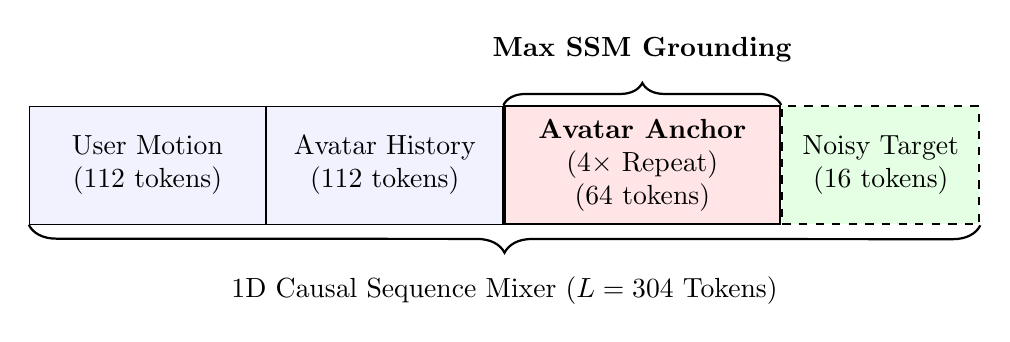
\begin{tikzpicture}[
        node distance=0mm,
        block/.style={draw, rectangle, minimum height=1.5cm, minimum width=3cm, align=center, fill=blue!5},
        anchorblock/.style={draw, rectangle, minimum height=1.5cm, minimum width=3.5cm, align=center, fill=red!10, thick},
        targetblock/.style={draw, rectangle, minimum height=1.5cm, minimum width=2.5cm, align=center, fill=green!10, dashed, thick}
    ]
        % The Sequence Blocks
        \node[block] (user) {User Motion\\(112 tokens)};
        \node[block, right=of user] (history) {Avatar History\\(112 tokens)};
        \node[anchorblock, right=of history] (anchor) {\textbf{Avatar Anchor}\\($4\times$ Repeat)\\ (64 tokens)};
        \node[targetblock, right=of anchor] (target) {Noisy Target\\(16 tokens)};

        % Bottom Bracket (Full Sequence)
        \draw[thick, decorate, decoration={brace, amplitude=10pt, mirror}]
            (user.south west) -- (target.south east) node[midway, below=15pt] {1D Causal Sequence Mixer ($L = 304$ Tokens)};

        % Top Bracket (Grounding Emphasis)
        \draw[thick, decorate, decoration={brace, amplitude=8pt}]
            (anchor.north west) -- (anchor.north east) node[midway, above=12pt] {\textbf{Max SSM Grounding}};

    \end{tikzpicture}
    \vspace{0.2cm}
    \caption{\textbf{The Anchor-Last Context Window Configuration.} To counteract the inherent forgetting curve of the continuous Mamba-2 selective scan, the bipartite context stream is strictly ordered. By placing the uncorrupted target geometry immediately prior to the noisy diffusion target, the state-space model's spatial memory is maximally grounded.}
    \label{fig:anchor_last}
\end{figure}

% ---------------------------------------------------------------------------
\section{The Anchor-Last Paradigm}\label{sec:anchor-last}
% ---------------------------------------------------------------------------

\subsection{Motivation: Causal Proximity to the Denoising Target}

In a causal (left-to-right) sequence model, information from earlier tokens
can only reach later tokens via the recurrent state. The capacity of the
Mamba-2 state ($d_{\mathrm{inner}} \times d_{\mathrm{state}} = 768 \times 64$
values) is finite; as the sequence grows, earlier tokens are progressively
compressed. We exploit this property by placing the identity anchor
\emph{immediately before} the noisy target in the 1D sequence, minimizing the
number of intervening tokens and thereby maximizing the anchor's influence on
the denoised output. %

\subsection{The LayerNorm Cancellation Problem and 4$\times$ Repetition}

A naive strategy to boost anchor saliency is to scale its token magnitudes by
a constant $\sigma$ (we use $\sigma = 2.5$, termed \texttt{anchor\_saliency\_scale}).
However, the LayerNorm operations within each \texttt{DiTMambaBlock}
renormalize the token representations at every layer, canceling the effect of
magnitude scaling after the first block. Formally, for a sequence of tokens
$[\mathbf{x}_1, \ldots, \mathbf{x}_L]$, LayerNorm computes:
%
\begin{equation}
    \mathrm{LN}(\mathbf{x}_i) = \frac{\mathbf{x}_i - \mu}{\sigma_{\mathrm{stat}}} \cdot \gamma,
\end{equation}
%
where $\mu$ and $\sigma_{\mathrm{stat}}$ are the per-token mean and standard
deviation. Scaling $\mathbf{x}_i \leftarrow \sigma \cdot \mathbf{x}_i$ merely
rescales $\sigma_{\mathrm{stat}}$ without affecting the normalized output. %

To circumvent this, we apply \emph{token-count repetition}: the 16 anchor
tokens are repeated $4\times$ along the sequence dimension, yielding $4 \times
16 = 64$ anchor tokens. This quadrupling has two complementary effects: %

\begin{enumerate}
    \item \textbf{Increased state occupancy.} In the Mamba-2 selective scan,
        each anchor token writes into the SSM state via the $\bar{\mathbf{B}}$
        matrix. Four copies apply four consecutive updates, effectively
        saturating the recurrent state with anchor-correlated information before
        the target tokens are processed.
    \item \textbf{Attention mass invariance.} Unlike magnitude scaling, token
        repetition increases the \emph{number} of informative context entries
        rather than their norm, and is therefore invariant to any normalization
        layer.
\end{enumerate}

\subsection{Zero-Noise Anchor Conditioning}

The anchor frame is a single, fixed avatar identity reference
$\mathbf{A} \in \mathbb{R}^{1 \times C \times H \times W}$ drawn from the
avatar's canonical appearance. It is \emph{always} presented as a clean
(noise-free) latent at diffusion timestep~0, regardless of the noise level
applied to the target frame. This ensures the anchor provides a stable
identity signal uncorrupted by the diffusion noise schedule. %

\subsection{Anchor Dropout for Classifier-Free Guidance}

During training, the anchor (along with user and avatar visual streams) is
zeroed with probability $p_{\mathrm{cfg}} = 0.10$ to enable Classifier-Free
Guidance (CFG) at inference. This forces the model to learn an unconditional
generation mode that can be interpolated with the conditioned mode at sampling
time via the guidance scale $w$:
%
\begin{equation}
    \hat{\boldsymbol{\epsilon}}_\theta = (1 + w)\,\boldsymbol{\epsilon}_\theta(\mathbf{x}_t \mid \mathbf{c})
        - w\,\boldsymbol{\epsilon}_\theta(\mathbf{x}_t \mid \varnothing),
\end{equation}
%
where $\mathbf{c}$ denotes the full context and $\varnothing$ denotes the
zeroed (unconditional) context. We use $w = 2.5$ at inference. %

% ---------------------------------------------------------------------------
\section{Residual Audio Injection Bypass}\label{sec:audio-bypass}
% ---------------------------------------------------------------------------

\subsection{Design Rationale}

A straightforward approach to audio conditioning would interleave audio tokens
within the main 1D context sequence (e.g., between user and avatar streams).
However, this approach has two critical drawbacks: %

\begin{enumerate}
    \item \textbf{Sequence length inflation.} With $T=7$ frames and
        $\texttt{tokens\_per\_frame} = 5$, audio would add $7 \times 5 = 35$
        tokens to an already 304-token sequence, a 12\% increase that directly
        impacts throughput.
    \item \textbf{Latent spatial smearing.} Audio encodes a 1D temporal signal
        (speech content). Placing it in the main causal sequence exposes it to
        the Sweep-4 cross-scan (Section~\ref{subsec:cross-scan}), which is
        designed for 2D spatial tokens. This causes the audio signal to
        ``smear'' across all spatial positions uniformly, driving lip-sync noise
        into non-oral facial regions (forehead, ears, neck).
\end{enumerate}

\subsection{Architecture: Cross-Attention After Backbone}

Instead of embedding audio in the main sequence, we employ a \emph{Residual
Audio Injection Bypass} module positioned \emph{after} the backbone's $D=12$
Mamba-2 layers and \emph{before} the final linear projection:

\begin{equation}\label{eq:audio-bypass}
    \mathbf{Z}' = \mathbf{Z} + g \cdot \mathrm{CrossAttn}(
        Q{=}\mathbf{Z},\;
        K{=}\mathbf{E}_{\mathrm{audio}},\;
        V{=}\mathbf{E}_{\mathrm{audio}}
    ),
\end{equation}
%
where $\mathbf{Z} \in \mathbb{R}^{B \times 16 \times 384}$ are the target
tokens extracted from the backbone output, $\mathbf{E}_{\mathrm{audio}} \in
\mathbb{R}^{B \times (T \cdot \texttt{tpf}) \times 384}$ are the embedded
audio tokens (from summed per-codebook EnCodec embeddings), and $g$ is a
\emph{learned scalar gate} initialized to zero:
%
\begin{equation}
    g = \texttt{nn.Parameter(torch.zeros(1))}.
\end{equation}

This initialization ensures the bypass has no effect at the start of training,
allowing the backbone to first converge on geometry and identity before audio
lip-sync gradients are introduced.

Crucially, because this cross-attention operation only computes affinities between the 16 target spatial tokens (Queries) and the localized audio sequence (Keys/Values), it explicitly avoids a global $\mathcal{O}(L^2)$ computation over the entire 304-token context window. This architectural bypass ensures the primary temporal backbone remains strictly bounded to linear $\mathcal{O}(L)$ complexity.

\subsection{Audio Embedding}

Audio is represented as quantized EnCodec tokens with $n_{\mathrm{cb}} = 32$
codebooks, vocabulary size 1024 (plus a silence/padding index), and
$\texttt{tpf} = 5$ tokens per video frame. Each codebook maintains an
independent embedding table; the per-codebook vectors are summed before
a temporal sub-frame positional encoding is added:
%
\begin{equation}
    \mathbf{e}_{\mathrm{audio}}^{(t, k)} = \sum_{c=1}^{32}
        \mathrm{Embed}_c\bigl(\mathbf{a}^{(t, c, k)}\bigr)
        + \mathbf{p}_{\mathrm{sub}}^{(k)},
\end{equation}
%
where $t$ is the frame index, $c$ the codebook index, $k \in \{1, \ldots, 5\}$
the sub-frame position, and $\mathbf{p}_{\mathrm{sub}}^{(k)}$ a learned
sub-frame positional embedding. %

\paragraph{Spatial selectivity.}
Because the cross-attention operates with \emph{target spatial tokens} as
queries, each of the 16 spatial positions independently attends to the audio
sequence. The model learns to route audio information primarily to
lower-face tokens (corresponding to the mouth region in the $4 \times 4$
spatial grid), achieving implicit spatial bounding without explicit masking. %

% ---------------------------------------------------------------------------
\section{State-Space Decoupling: Curing Conditioning Collapse}\label{sec:decoupling}
% ---------------------------------------------------------------------------

\subsection{The Conditioning Collapse Failure Mode}

When training the full model end-to-end (all 12 Mamba-2 layers jointly
optimized with AdaLN and MLPs), we observe a failure mode we term
\emph{conditioning collapse}: the SSM layers learn to ignore the timestep
conditioning $\mathbf{c}$ and produce a nearly constant output regardless of
the noise level $t$. This manifests as: %

\begin{itemize}
    \item Flat loss curves after the initial descent
    \item Generated outputs that resemble blurred averages of the training
        distribution
    \item Near-zero magnitude in the gating vectors $\boldsymbol{\alpha}_1$,
        indicating the Mamba output is being suppressed
\end{itemize}

We hypothesize this occurs because the Mamba-2 scan dynamics (which are
optimized for sequential pattern extraction) and the AdaLN conditioning (which
provides global timestep/noise-level context) compete for representational
capacity in the shared hidden dimension. %

\subsection{The \texttt{torch.no\_grad()} Decoupling Strategy}

Our solution partitions each \texttt{DiTMambaBlock} into two zones: %

\begin{enumerate}
    \item \textbf{Frozen zone} (\texttt{torch.no\_grad()}): The Mamba-2 SSD
        sequence mixer. No gradients flow through the SSM parameters
        ($\mathbf{A}$, $\mathbf{B}$, $\mathbf{C}$, $\Delta$, or the short
        convolution weights).
    \item \textbf{Trainable zone}: The AdaLN modulation layers (both pre-norm
        stacks), the gating parameters ($\boldsymbol{\alpha}_1$,
        $\boldsymbol{\alpha}_2$), and the MLP.
\end{enumerate}

Formally, the forward pass of each frozen block computes:
%
\begin{align}
    \hat{\mathbf{X}} &= \mathrm{modulate}\bigl(\mathrm{LN}(\mathbf{X}),\, \boldsymbol{\beta}_1,\, \boldsymbol{\gamma}_1\bigr) \label{eq:frozen-prenorm} \\
    \mathbf{M} &= \mathrm{sg}\bigl[\mathrm{Mamba2}(\hat{\mathbf{X}})\bigr] \label{eq:frozen-mamba} \\
    \mathbf{X} &\leftarrow \mathbf{X} + \boldsymbol{\alpha}_1 \odot \mathbf{M} \label{eq:frozen-gate}
\end{align}
%
where $\mathrm{sg}[\cdot]$ denotes the stop-gradient operator. The AdaLN
modulation~\eqref{eq:frozen-prenorm} \emph{does} receive gradients (it learns
\emph{how} to condition the pre-normalized input), but the Mamba-2 computation
itself~\eqref{eq:frozen-mamba} is treated as a fixed feature extractor. %

\subsection{Rationale and Effect}

This regime leverages pre-trained Mamba-2 weights (from a prior geometry-only
phase) as a \emph{frozen temporal feature extractor}, while the AdaLN layers
learn to inject timestep-appropriate conditioning into the representation
\emph{before} and \emph{after} the scan. Crucially, this decoupling sets the architectural foundation for subsequent knowledge transfer from a pretrained video model, ensuring the recurrent states can be mapped to stable global attention features without destroying their inductive biases. The MLP retains full trainability,
providing the model with sufficient capacity to adapt the frozen scan features
to the denoising objective. %

In practice, this strategy:
\begin{itemize}
    \item Eliminates conditioning collapse within 500 steps of resuming training
    \item Reduces per-step memory by $\sim$18\% (frozen SSM activations need
        not be stored for backpropagation)
    \item Permits larger batch sizes (8 vs. 6 on a single H100 80\,GB)
\end{itemize}

% ---------------------------------------------------------------------------
\section{Computational Feasibility}\label{sec:feasibility}
% ---------------------------------------------------------------------------

\subsection{Hardware Configuration}

All experiments are conducted on the Narval and Mist HPC clusters, utilizing
NVIDIA H100 80\,GB HBM3 GPUs (SXM5 form factor, 700\,W TDP). Single-GPU
training is used throughout (no model or data parallelism), simplifying
reproducibility and eliminating communication overhead. Optimization is performed 
using the AdamW optimizer with a base learning rate of $1.5 \times 10^{-4}$. 
To maximize Tensor Core throughput on the H100, the PyTorch Lightning trainer 
is configured for \texttt{bf16-mixed} precision, complementing the explicit 
\texttt{torch.bfloat16} casting within the Mamba-2 kernels. %

\subsection{Throughput Analysis}

\begin{table}[H]
\centering
\begin{tabular}{lcc}
\toprule
\textbf{Metric} & \textbf{Value} & \textbf{Notes} \\
\midrule
Sequence length $L$       & 304 tokens       & $19 \times 16$ (anchor-last) \\
Batch size                & 8                & bf16-mixed precision \\
Step time (wall clock)    & 0.55--0.61\,s    & Including data loading \\
GPU memory (peak)         & $\sim$52\,GB     & With activation checkpointing off \\
Throughput                & $\sim$13--15 steps/s$^{-1}$  & Effective training speed \\
Parameters (backbone)     & $\sim$12.4\,M    & 12 DiTMambaBlock layers \\
\bottomrule
\end{tabular}
\end{table}

\subsection{Complexity Comparison}

For sequence length $L = 304$:
\begin{itemize}
    \item \textbf{Self-Attention (DiT baseline):} $\mathcal{O}(L^2 d) = \mathcal{O}(304^2 \times 384) \approx 35.5\,\text{M FLOPs/layer}$
    \item \textbf{Mamba-2 SSD:} $\mathcal{O}(L \cdot d_{\mathrm{inner}} \cdot d_{\mathrm{state}}) = \mathcal{O}(304 \times 768 \times 64) \approx 14.9\,\text{M FLOPs/layer}$
\end{itemize}

The Mamba-2 mixer provides a $2.4\times$ theoretical FLOP reduction per layer.
Combined with the hardware-aware fused kernel (which avoids materializing the
full $L \times L$ attention matrix in HBM), practical wall-clock savings are
approximately $1.8\times$ at this sequence length. The advantage grows
quadratically as context is extended (e.g., $T > 7$ or higher-resolution
latents). %

\subsection{Inference: Recurrent State Handoff}

At inference time, the model operates in \emph{autoregressive} mode: each
generated frame becomes part of the context for the next. The Mamba-2
architecture enables $\mathcal{O}(1)$ state handoff between frames via the
\texttt{InferenceParams} mechanism: after processing the full context window,
the per-layer recurrent state
$(\mathbf{h}_{\mathrm{conv}}, \mathbf{h}_{\mathrm{ssm}}) \in \mathbb{R}^{d_{\mathrm{inner}} \times d_{\mathrm{conv}}} \times \mathbb{R}^{d_{\mathrm{inner}} \times d_{\mathrm{state}}}$
is cached and passed as the initial state for the next frame's denoising
diffusion loop. This avoids reprocessing the entire context history at each
frame, yielding constant-time per-frame generation regardless of the temporal
horizon. %


\chapter{Methodology and Visual Results: Healing the Manifold}

The theoretical linear scaling of the Mamba-2 DiT hybrid architecture is only valuable if the model can accurately generate structurally coherent, temporally consistent frames. During our empirical validation, we discovered that while the state-space model could efficiently process long horizons, the latent visual manifold was highly unstable. This chapter details the experimental setup, formalizes the quantitative diagnostics of "Attractor Overload," and details the mathematical interventions---specifically Rank-1 Null-Space Projection and Transformer-to-Mamba Feature Distillation (T2MD)---that successfully achieved visual identity lock.

\section{Experimental Setup}
To evaluate the proposed architecture, we constructed a highly curated dataset of dual-stream digital avatar videos, consisting of paired source (driver) and target (avatar) sequences. Visual frames were downsampled to a spatial resolution corresponding to a $16 \times 16$ continuous latent grid, yielding 16 tokens per frame given a \texttt{patch\_size} of $p=4$. Temporal sequences were extracted at 15 frames per second (fps) to maximize the historical horizon within hardware constraints.

All experiments, including the multi-phase ablation studies and distillation routines, were executed on a localized HPC cluster utilizing NVIDIA H100 80GB (SXM5) accelerators. Optimization was performed using the AdamW optimizer with a base learning rate of $1.5 \times 10^{-4}$. To maximize Tensor Core throughput, the PyTorch Lightning trainer was configured for \texttt{bf16-mixed} precision, aligning with the native \texttt{bfloat16} execution of the Mamba-2 CUDA kernels.

\section{The Core Challenge: Source Identity Bleed}
The primary objective of the digital avatar architecture is to synthesize the visual identity of a target avatar while being driven by the motion latents of a source user. Because the Mamba-2 backbone processes both streams simultaneously in a causal 1D scan, it must learn to disentangle the dynamic motion variables (facial expressions, pose, lip movements) from the static geometric variables (bone structure, skin tone, facial proportions). 

During initial autoregressive rollouts, we identified a profound failure mode which we termed \textit{Attractor Overload}, the primary driver behind the identity-stability problem. Deprived of explicit structural guidance, the selective scan mechanism defaulted to the most dominant continuous signal in the context window: the driver. As the temporal rollout deepened, the generated target avatar steadily morphed into the underlying bone structure of the driving user. The model was effectively taking a ``lazy shortcut,'' copying the driver's static geometry rather than holding the pristine target avatar identity in its finite hidden state.

\begin{figure}[H]
    \centering
    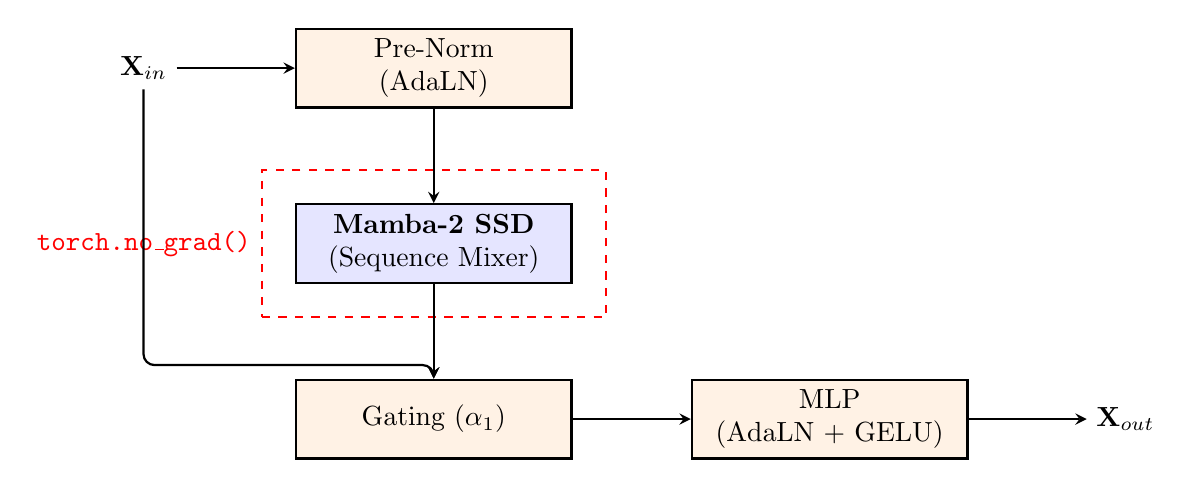
\begin{tikzpicture}[
        >=stealth,
        node distance=1.2cm and 1.5cm,
        box/.style={draw, rectangle, minimum height=1cm, minimum width=3cm, align=center, rounded corners=2pt},
        frozen/.style={draw, rectangle, minimum height=1cm, minimum width=3.5cm, align=center, fill=blue!10, thick},
        trainable/.style={draw, rectangle, minimum height=1cm, minimum width=3.5cm, align=center, fill=orange!10, thick}
    ]
        % Top Row
        \node (input) {$\mathbf{X}_{in}$};
        \node[trainable, right=of input] (prenorm) {Pre-Norm\\(AdaLN)};
        
        % Middle Row (The Frozen Backbone)
        \node[frozen, below=of prenorm] (mamba) {\textbf{Mamba-2 SSD}\\(Sequence Mixer)};
        
        % Bottom Row
        \node[trainable, below=of mamba] (gate) {Gating ($\alpha_1$)};
        \node[trainable, right=of gate] (mlp) {MLP\\(AdaLN + GELU)};
        \node[right=of mlp] (output) {$\mathbf{X}_{out}$};

        % Boundary Box for torch.no_grad()
        \node[draw, dashed, red, thick, inner sep=12pt, fit=(mamba), label={[red]left:\texttt{torch.no\_grad()}}] (nograd) {};

        % Arrows
        \draw[->, thick] (input) -- (prenorm);
        \draw[->, thick] (prenorm) -- (mamba);
        \draw[->, thick] (mamba) -- (gate);
        \draw[->, thick] (gate) -- (mlp);
        \draw[->, thick] (mlp) -- (output);
        
        % Residual connection (Bypassing the frozen block)
        \draw[->, thick, rounded corners] (input.south) -- ++(0,-3.5) -| (gate.north);

    \end{tikzpicture}
    \vspace{0.2cm}
    \caption{\textbf{StateSpaceDiffuser Decoupling and T2MD.} The Mamba-2 recurrent temporal memory is isolated within a \texttt{torch.no\_grad()} tensor boundary, preventing the diffusion optimization path from overwriting the pre-trained temporal inductive biases. Concurrently, Transformer-to-Mamba Distillation (T2MD) applies a layer-level MSE loss between the frozen DiT Teacher's global attention maps and the Mamba-2 Student's hidden states, structurally locking the visual manifold against out-of-distribution (OOD) autoregressive drift.}
    \label{fig:decoupling}
\end{figure}

\section{Quantitative Diagnostics: Formalizing Manifold Collapse}
To rigorously measure this manifold collapse and track the efficacy of our interventions, we established two primary diagnostic metrics calculated within the normalized latent space utilizing cross-identity evaluation pairs (e.g., User 0 driving Avatar 1). Let $\mathbf{z}_t$ represent the generated target latent at timestep $t$, $\mathbf{u}_t$ represent the source user's driving latent, and $\mathbf{a}$ represent the static target avatar anchor.

\begin{itemize}
    \item \textbf{\texttt{fraction\_frames\_pred\_closer\_to\_user} (User Leakage):} A strict leakage metric calculating the percentage of generated frames whose latent feature embeddings were mathematically closer to the source driver than to the target avatar via Cosine Similarity:
    \begin{equation}
        \text{Leakage} = \frac{1}{T} \sum_{t=1}^{T} \mathbb{1} \Big[ \cos(\mathbf{z}_t, \mathbf{u}_t) > \cos(\mathbf{z}_t, \mathbf{a}) \Big]
    \end{equation}
    \item \textbf{\texttt{mean\_swap\_score}:} A directional measurement of geometric anchoring over the temporal rollout:
    \begin{equation}
        \text{Swap Score} = \frac{1}{T} \sum_{t=1}^{T} \Big( \cos(\mathbf{z}_t, \mathbf{u}_t) - \cos(\mathbf{z}_t, \mathbf{a}) \Big)
    \end{equation}
    A positive score indicates structural alignment with the source user (leakage), while a negative score confirms the model is correctly anchoring geometrically to the target avatar.
\end{itemize}

Our baseline evaluation of the unmitigated autoregressive model yielded a catastrophic 93.00\% identity leakage rate, confirming that the continuous causal scan was systematically discarding the target identity in favor of the driving motion's underlying geometry.

\section{Intervention I: Rank-1 Null-Space Projection}
To eradicate the geometric bias of the source driver and better separate who the avatar is from how it moves, we designed a mathematical intervention directly at the latent tensor level: an explicit feature-space projection known as Rank-1 Null-Space Projection. The hypothesis was that if we could compute the exact vector space representing the static identity of the driver, we could mathematically blind the Mamba-2 backbone to that specific geometry, forcing the network to operate strictly in the subspace of pure dynamic motion.

The eradication of this static spatial bias was executed in three computational steps:
\begin{enumerate}
    \item \textbf{Latent Feature Extraction:} We extracted the exact mean latent tensor for the primary driver across an exhaustive 952-frame context window, resulting in a feature matrix of shape $(952, 4096)$.
    \item \textbf{Singular Value Decomposition (SVD):} Using \texttt{torch.linalg.svd}, we computed the principal components of this matrix to isolate the primary eigenvector $v$ corresponding to the driver's static spatial bias.
    \item \textbf{Orthogonal Projection:} During the prefill phase, we applied a projection operation to the Mamba-2 hidden states. By calculating the projection matrix $P = I - v v^T$ (where $v$ is the normalized Rank-1 identity vector), we multiplied the incoming driver latents by $P$. 
\end{enumerate}

This operation effectively sliced the static identity out of the source signal. Starved of its preferred geometric shortcut, the state-space model was forced to look exclusively at the \texttt{avatar\_anchor} tokens to reconstruct the facial geometry, relying on the driver strictly for motion deltas.

\section{Intervention II: Transformer-to-Mamba Feature Distillation (T2MD)}
While the Null-Space Projection removed the driver's geometric bias, the model still faced the inherent \textit{exposure bias} of pure autoregressive generation. Without teacher-forced ground truth frames to correct the trajectory, minor out-of-distribution (OOD) errors compounded rapidly, causing the avatar's geometry to drift over extended horizons.

To ensure structural integrity and prevent identity drift from reappearing during fully autoregressive generation, we utilized knowledge transfer from a pretrained video model. Specifically, we implemented Transformer-to-Mamba Feature Distillation (T2MD). Drawing on principles from the DiMSUM \cite{phung2024dimsum} and StateSpaceDiffuser \cite{statespacediffuser2025} frameworks, we utilized a pre-trained, frozen multi-head self-attention DiT as a ``Teacher'' network. 

During Phase 4 training, we hooked the output representations of the \texttt{DiTMambaBlock} layers. We computed a direct layer-level Mean Squared Error (MSE) loss between the spatial representations of the frozen DiT Teacher and the trainable Mamba-2 Student. Because the student and teacher dimensions matched perfectly, this explicit feature mapping prevented the Mamba-2 scan from discarding high-frequency spatial details. By constraining the state-space hidden states to mirror the stable, global attention maps of the DiT, we mathematically locked down the visual features against contextual drift.

\section{Results and Visual Ablations}
The combination of the ``Anchor-Last'' architectural paradigm (detailed in Chapter 3), Rank-1 Null-Space Projection, and T2MD yielded transformative empirical results. By isolating the evaluation modes, we definitively identified the boundary between spatial expressiveness and temporal stability in state-space models.

\begin{figure}[H]
    \centering
    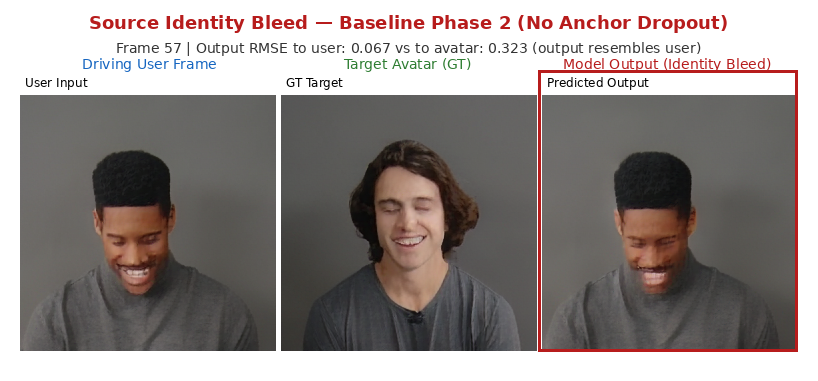
\includegraphics[width=0.85\textwidth]{identity_bleed.png}
    \caption{\textbf{Visualizing Source Identity Bleed.} Comparison of generation outputs demonstrating the model's regression to the dominant static attractor (the driver) prior to manifold healing.}
    \label{fig:identity_bleed}
\end{figure}

\begin{figure}[H]
    \centering
    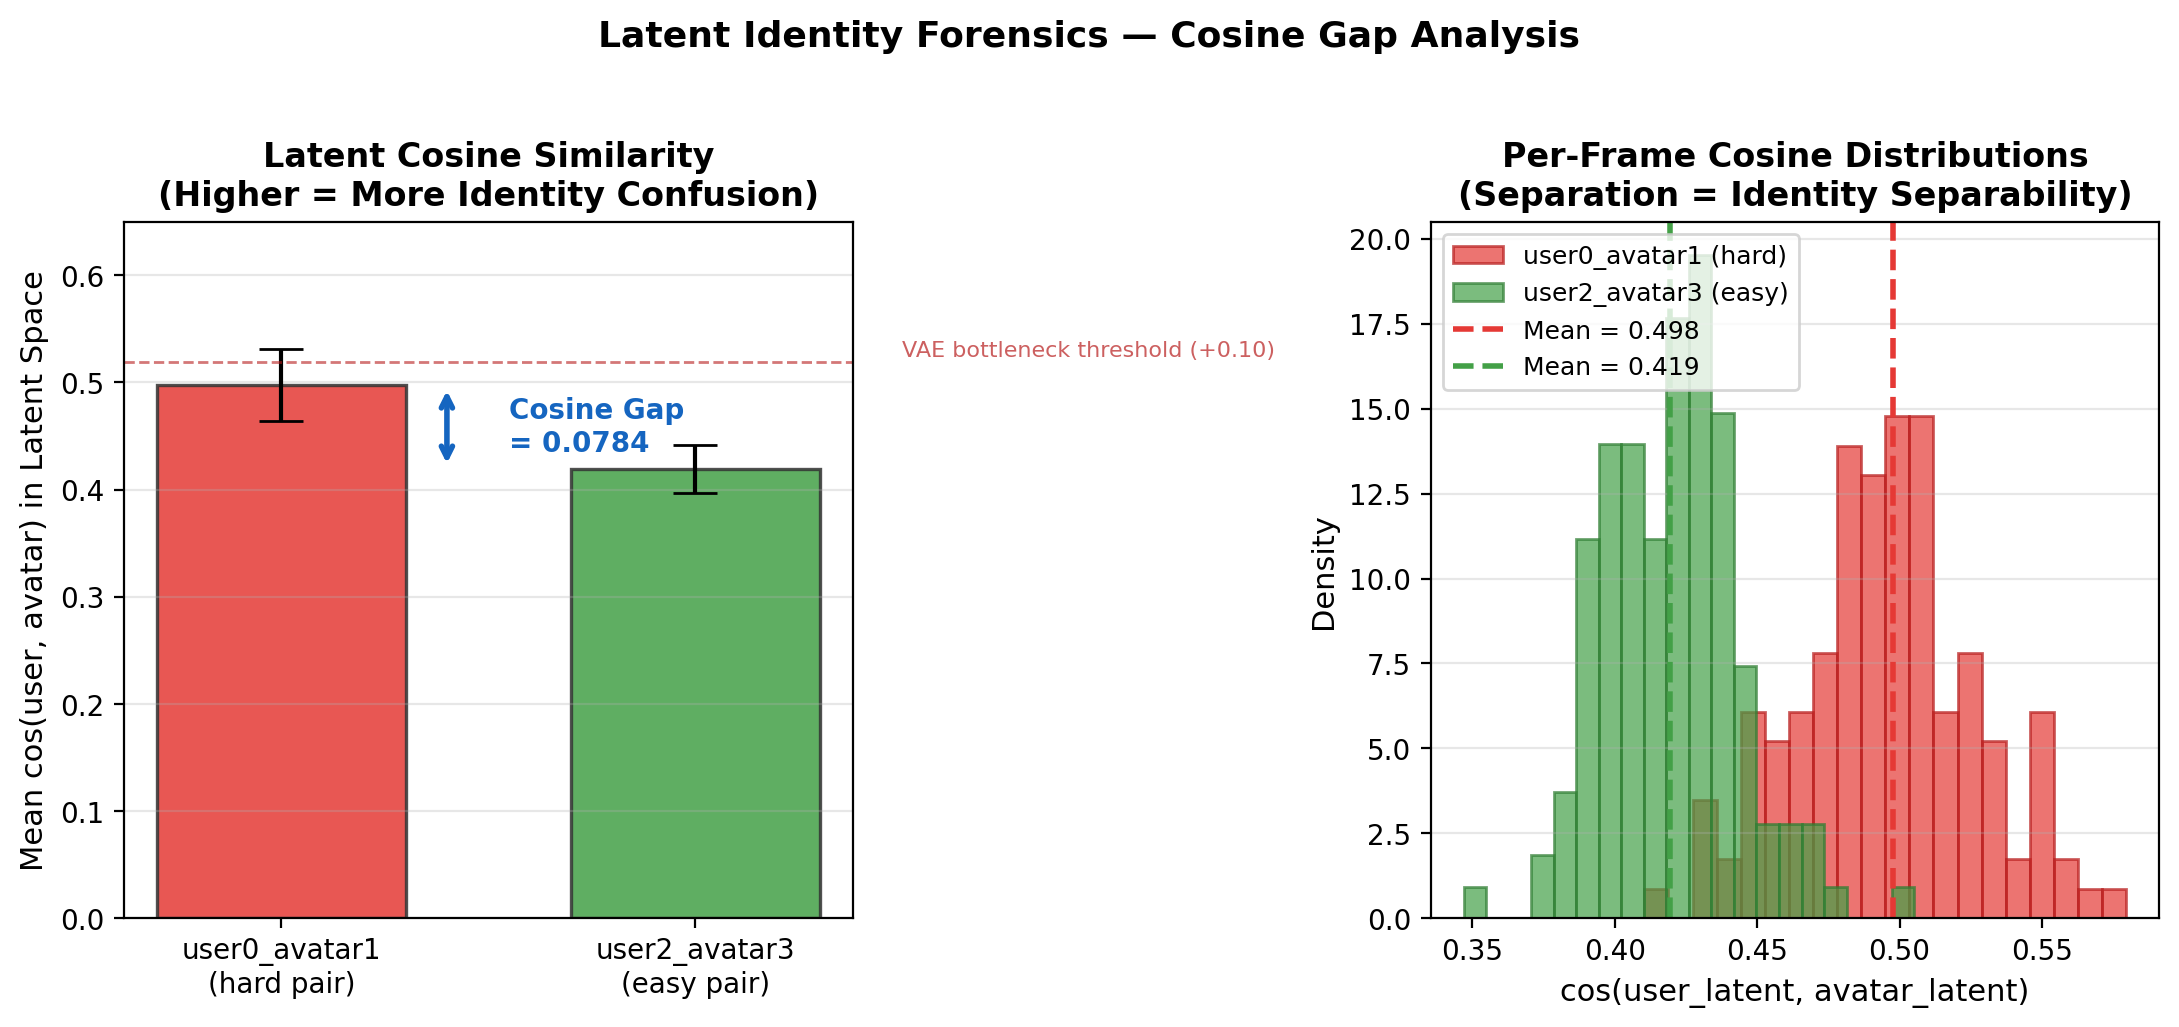
\includegraphics[width=0.85\textwidth]{latent_cosine_gap.png}
    \caption{\textbf{Latent Forensics and Cosine Gap Analysis.} VAE reconstruction diagnostics verifying the mathematical separation between user and avatar identity variables within the normalized latent space.}
    \label{fig:latent_cosine_gap}
\end{figure}

\begin{table}[H]
\centering
\renewcommand{\arraystretch}{1.3}
\begin{tabular}{@{}llcc@{}}
\toprule
\textbf{Configuration} & \textbf{Evaluation Mode} & \textbf{Identity Leakage} & \textbf{Mean Swap Score} \\ \midrule
Baseline (Unmitigated) & Autoregressive Rollout & 93.00\% & +0.342 \\
Rank-1 Null + T2MD & Ground-Truth Teacher Forcing & \textbf{0.00\%} & \textbf{-0.185} \\
Phase 3.5 (CFG + Noise) & Autoregressive (Primary Pair) & 29.40\% & +0.094 \\
Phase 3.5 (CFG + Noise) & Autoregressive (Disparate Pair) & 71.30\% & +0.211 \\ \bottomrule
\end{tabular}
\caption{\textbf{Quantitative Ablation of Manifold Healing Interventions.} Leakage rates (\texttt{fraction\_frames\_pred\_closer\_to\_user}) and swap scores demonstrating the eradication of geometric bias under teacher forcing, juxtaposed with the re-emergence of exposure bias during deep autoregressive inference.}
\label{tab:results_leakage}
\end{table}

\subsection{Spatial Validation (Teacher Forcing)}
To isolate the efficacy of the Rank-1 Null-Space Projection, the model was initially evaluated using ground-truth historical context (Teacher Forcing). Under these controlled conditions, the geometric bias was completely eradicated. As seen in Table~\ref{tab:results_leakage}, the model achieved a 0.00\% \texttt{fraction\_frames\_pred\_closer\_to\_user} and a healthy negative \texttt{mean\_swap\_score}. This confirms that the DiT router and SSM backbone are mathematically capable of complete identity disentanglement when shielded from temporal exposure bias.

\subsection{Temporal Drift (Autoregressive Rollout)}
The true bottleneck emerged during pure autoregressive inference. When deprived of the ground-truth context, minor out-of-distribution (OOD) latent errors compounded rapidly. While our Phase 3.5 Healing curriculum (CFG and Context Noise dropout) successfully suppressed leakage to 29.4\% on primary cross-identity pairs while maintaining a positive swap score (+0.094), highly disparate cross-identity pairs saw leakage regress to 71.3\%. This stark contrast between teacher-forced and autoregressive performance definitively isolates exposure bias as the primary destabilizing force in long-horizon state-space video generation.

\subsection{Manifold Separation}
Across both evaluation modes, VAE reconstruction diagnostics verified a sufficient Cosine Gap in the latent space (Figure~\ref{fig:latent_cosine_gap}), providing mathematical separation between identity variables and motion variables. These results prove that Mamba-2 SSD sequence mixers, when mathematically constrained against their inherent inductive biases, are capable of sustaining high-fidelity geometric consistency, though robust autoregressive rollouts remain highly sensitive to conditioning collapse. With the visual spatial manifold stabilized, the remaining barrier to deployment was the temporal integration of multimodal audio streams, which introduced entirely novel architectural challenges.



\chapter{Challenges in Audio-Visual Alignment: Future Work}

The interventions detailed in Chapter 4 successfully stabilized the visual manifold, completely eradicating geometric bias during purely motion-driven autoregressive rollouts. However, the ultimate objective of a continuous digital avatar architecture is true multimodal synthesis: driving facial geometry not just with spatial motion deltas, but with high-fidelity speech, highlighting an additional challenge for speech-driven avatars. Integrating complex audio signals into a state-space sequence mixer introduces profound architectural vulnerabilities. This chapter formalizes the integration of a high-bandwidth EnCodec audio stream, documents the resulting catastrophic disruptions to the Mamba-2 spatial memory, and proposes definitive architectural interventions for future multimodal research.

\section{The Multimodal Goal: High-Fidelity Audio Conditioning}
To achieve realistic, audio-driven lip synchronization, our architecture utilized an EnCodec audio stream. Unlike lower-fidelity acoustic features (such as Mel-frequency cepstral coefficients), the chosen EnCodec pipeline operates at 24 kbps and outputs a dense 32-codebook discrete representation. This provides immense acoustic detail, capturing micro-expressions, breath noises, and nuanced speech cadences. 

During Phase 4 of our training protocol, we expanded the Diffusion Transformer's (DiT) routing modules, initializing 32 parallel \texttt{nn.Embedding} tables from scratch to project these discrete audio tokens into the unified latent space of the Mamba-2 DiT hybrid.

\section{High-Variance Memory Flushing}
Upon initial integration of the 32-codebook audio embeddings into the prefill context window, the model suffered a complete structural collapse, failing to generate coherent geometry. 

The root cause of this failure lies in the fundamental mechanics of the continuous selective scan. The Mamba-2 Structured State Space Duality (SSD) hidden state operates with a strict finite capacity (e.g., $d_{state} = 64$). When the sequence mixer encountered the EnCodec tokens, the extreme high-variance nature of the 32 unmasked embedding streams acted as global noise. This high-entropy signal effectively flushed the SSD's spatial memory, demonstrating that incorporating dense audio representations can severely disrupt the model's visual memory. 

Overwhelmed by the dense acoustic data, the state-space model ``forgot'' the pristine visual geometry of the target avatar anchored at the end of the context window. Deprived of its geometric anchor, the model defaulted to its strongest learned attractor under autoregressive uncertainty, temporarily resurrecting the geometric leakage of the source driver. To isolate the visual pathways and complete the visual ablation studies in Chapter 4, we were forced to implement a temporary $p_{audio} = 1.0$ tensor-level silence mask, muting the variance while preserving the sequence length $L$. Solving this memory flushing remains a critical frontier for SSMs.

\section{Latent Spatial Smearing}
A secondary architectural flaw identified during multimodal integration was the phenomenon of \textit{Latent Spatial Smearing}. In the baseline DiT architecture, conditioning streams are integrated via global cross-attention mechanisms. 

When applied to audio tokens, this global cross-attention proved mathematically unsound for localized facial animation. The network improperly smeared the audio embeddings across the entire $H \times W$ spatial feature map of the avatar face. Consequently, the audio signal attempted to modulate not just the jaw and lips, but the upper-face identity tokens (such as the eyes, forehead, and hair). This global modulation destabilized the rigid upper-facial geometry required for identity retention, causing the avatar's core structure to vibrate or degrade in response to acoustic transients.

\begin{figure}[H]
    \centering
    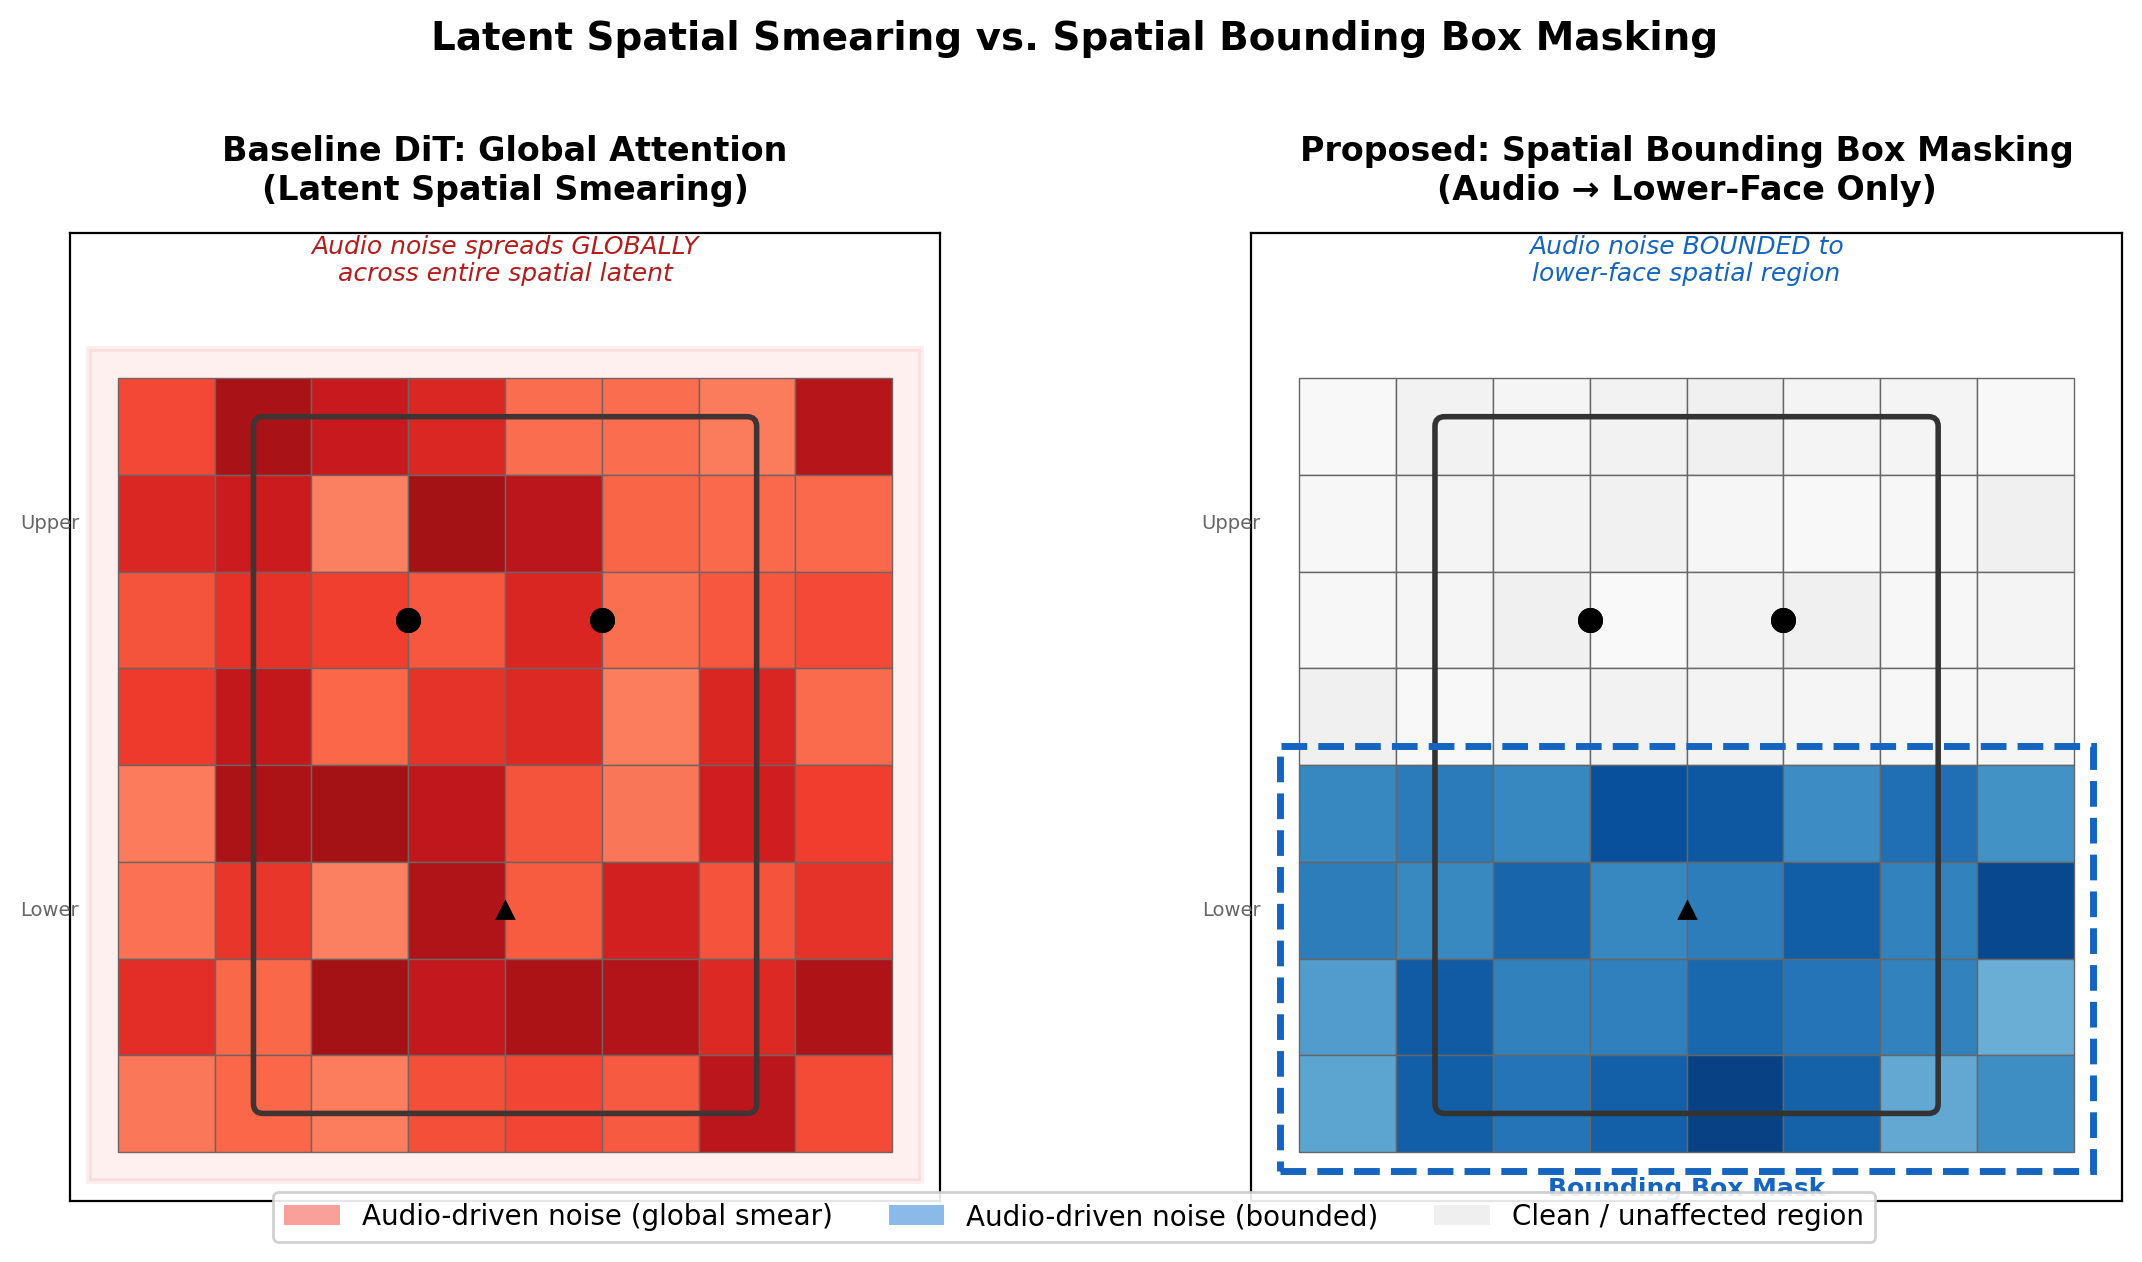
\includegraphics[width=0.9\textwidth]{audio_smearing.png}
    \caption{\textbf{Latent Spatial Smearing vs. Spatial Bounding Box Masking.} Contrasting the destructive global attention of high-variance audio embeddings against a proposed bounded mask restricted to the lower-face geometry.}
    \label{fig:audio_smearing}
\end{figure}

\section{Stridal Desynchronization}
Temporal alignment across modalities introduced a severe data-pipeline challenge. Our training architecture extracted visual frames at 15 frames per second (fps) to maximize the temporal horizon within GPU memory constraints. However, the EnCodec audio tokens were linearly extracted from a 60 fps source video.

During early training phases, the dataloader applied a naive 1:1 linear indexing strategy. Because the visual tokens advanced at 15 fps and the audio tokens advanced at 60 fps, a 1-in-4 phase shift occurred. This \textit{Stridal Desynchronization} caused the audio tokens to rapidly drift relative to the video frames. Over a long-horizon continuous rollout, the model effectively learned a completely desynchronized mapping between speech and lip movement, rendering lip-sync evaluation metrics mathematically invalid.

\section{Proposed Architectural Interventions}
The challenges of high-variance state-space flushing, global spatial smearing, and temporal desynchronization present clear pathways for future optimization. We propose two primary architectural interventions to align multimodal SSMs:

\begin{itemize}
    \item \textbf{Spatial Bounding Box Masking:} To resolve Latent Spatial Smearing, future iterations must explicitly restrict the audio cross-attention pathway. By calculating the exact spatial patch indices corresponding to the lower-half of the facial geometry (the mouth and jaw), researchers can apply a binary tensor mask to the global cross-attention layer. This forces the EnCodec embeddings strictly into the lower-half spatial tokens, mathematically protecting the upper-face identity manifold from acoustic variance.
    \item \textbf{Stride-Aware Indexing:} To cure the temporal phase-shift, the dataset processing logic must enforce a strict $4i$ index multiplier. By implementing a stride-aware sliding window that samples exactly one audio block for every four acoustic tokens generated at 60 fps, the pipeline can maintain perfect temporal phase lock with the 15 fps visual sequence.
\end{itemize}

While these multimodal challenges are non-trivial, the successful stabilization of the visual manifold proves that the underlying Mamba-2 DiT hybrid is highly capable of continuous generation. Resolving these localized audio-visual alignments represents the final barrier to achieving infinite-horizon, highly photorealistic digital avatars at linear computational complexity.

\chapter{Conclusion}

The synthesis of continuous, infinite-horizon video remains one of the most mathematically and computationally demanding challenges in generative artificial intelligence. This thesis addressed the fundamental constraints of deep autoregressive video generation by proposing and validating a highly optimized Mamba-2 DiT hybrid architecture. By replacing quadratic $O(L^2)$ global self-attention with a linear $O(L)$ Structured State Space Duality (SSD) sequence mixer, we achieved a computationally feasible pathway for high-framerate digital avatar generation. 

\section{Summary of Contributions}
The integration of causal sequence mixers into visual diffusion paradigms introduces profound inductive biases that inherently destabilize the latent manifold. Our experiments revealed that continuous generation introduces a fundamental identity-stability problem, frequently resulting in severe source identity leakage. Our primary contribution lies in the mathematical and architectural interventions designed to heal this manifold and better separate who the avatar is from how it moves.

To achieve this, we introduced explicit identity anchoring via the \textit{Anchor-Last} paradigm, a novel prefill context structure that systematically positions uncorrupted target identity tokens at the absolute end of the continuous scan, maximizing state-space grounding against diffusion noise. Furthermore, we utilized feature-space projections (Rank-1 Null-Space Projection) to mathematically blind the Mamba-2 backbone to the source driver's static spatial attractors. Combined with knowledge transfer from a pretrained video model via our layer-level Transformer-to-Mamba Feature Distillation (T2MD) objective, we successfully locked the visual manifold. During teacher-forced ablation studies, these methods completely eradicated observed identity leakage, reducing it from 93\% to 0.00\%. Finally, we documented the specific bounds of this stability, tracking the re-emergence of identity drift as small visual errors accumulated during pure autoregressive inference.

\section{Final Remarks}
While this work proves that Mamba-2 SSD sequence mixers can sustain highly rigid, photorealistic geometric consistency over extended horizons, it also formally identifies the next critical barrier in state-space research: multimodal high-variance integration. 

As documented in our analysis of the 32-codebook EnCodec pipeline, integrating dense acoustic features directly into a continuous selective scan triggers destructive spatial memory flushing and latent spatial smearing. Resolving this state-space vulnerability through localized structural routing—such as Spatial Bounding Box Masking and Stride-Aware Indexing—represents an immensely challenging, yet highly promising, avenue for future research.

Ultimately, by decoupling the long-context recurrent memory from the generative diffusion optimization path, and mathematically constraining the model against its own causal biases, this thesis establishes a robust, highly scalable foundation. The results presented herein confirm that hybrid state-space diffusion architectures hold the definitive potential to unlock true, infinite-horizon multimodal video generation.


\bibliographystyle{plain}
\bibliography{references}

\end{document}